\chapter{序論}
\label{chap:introduction}
\section{Service Function Chaining}
\label{section:sfc}

SFC とは,エンドツーエンド通信を提供するために必要なさまざまなサービスファンクション (SF) を決定及び順序付けし,それらを介するようにトラフィックを操作することを指す.
図~\ref{fig:sfc-arc} に,SFC アーキテクチャの概略図を示す.
SF には,ファイアウォールや IP ネットワークアドレストランスレータ (NAT) などのネットワークサービスファンクションや,アプリケーション固有の機能が含まれる.
SFC アーキテクチャは,基礎となるネットワークトポロジから独立したトポロジを前提としている.
この基礎となるネットワークトポロジをアンダーレイネットワークといい,独立した SFC のためのネットワークトポロジをオーバレイネットワークという.
図~\ref{fig:sfc-arc} では灰点線のパスを物理的なパスであるアンダーレイネットワークを示し,その他の実線を SFC として選択可能なパスの例であるオーバレイネットワークを示している.
SFC アーキテクチャでは,パケットは通信の入口となるノードで事前に定義されたポリシとパケット内の情報から分類され,SFC 対応ドメイン内で適用する SF のセットを決める.
その後,任意の順番で各 SF でパケット処理が適用されるように転送される.
例えば,Logging をした後 FW Service を適用,Filtering を適用すような場合は緑のパスを辿るようになる.

SFC アーキテクチャは,ネットワークの用途や運用計画などのコンテキストに依存しない,汎用的な場面で利用可能な技術である.
つまり,SFC アーキテクチャは固定ネットワークやモバイルネットワーク,多くのデータセンターアプリケーションに適用できる.
SFC の構築に関して,すべての SF が満たさなければならない標準の定義や特性は存在しない.
各 SF は単に「パケットに対する特定の処理を適用できる要素」として扱われ,特定のネットワークで常に有効な SF を静的に列挙することはできない.
なぜなら,適用する SF の集合はその瞬間に有効な SF であり,それらが有効かどうかはその時々のネットワーク環境によって異なる場合があるからである.
SF のチェインとそれらを呼び出す基準は,SF 対応ドメインを運用する各ネットワーク毎に固有である.

SFC における SF は,受信したパケットの特定の処理を担当する機能である.
SF はプロトコルスタックのさまざまなレイヤで動作し,論理的なコンポーネントとして仮想要素として実現されることもあれば,物理的な筐体としてネットワークの中に組み込まれることもある.
近年では,SF が動作するマシンは物理的な筐体ではなく,汎用マシンにインストールされたハイパーバイザ上の VM の中で動作することも多い.
また,コンテナ技術の台頭により,SF 自体をコンテナに閉じ込めてデプロイすることも一般的になっている.
さらに,それらのコンテナを kubernetes~\cite{k8s} に代表されるコンテナオーケストレータによって管理する手法も提案されている~\cite{sfc-with-k8s}
このように,仮想化されたネットワーク上の機能 (Network Function / NF) を NFV という.
SFC は NFV の利用例として NFV のコンテキストでも研究されてきた技術である.

\begin{figure}[t]
    \centering
    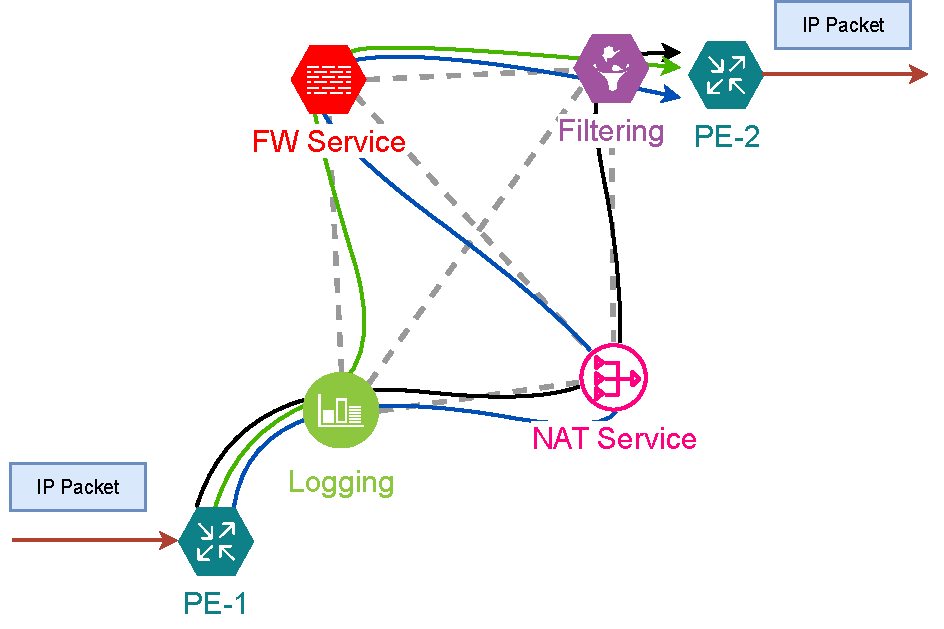
\includegraphics[width=0.95\linewidth]{img/SFC.pdf}
    \caption{SFC Architecture}
    \label{fig:sfc-arc}
\end{figure}

\section{従来のパケットルーティングとトラフィックエンジニアリング}
\label{section:src-rtng}

章\ref*{section:sfc} で述べた通り,SFC を実現するためには,エンドツーエンド通信を提供するために必要な複数の SF を決定,及び順序付けし,それらを介するようにトラフィックを操作する必要がある.
しかし,従来のパケットルーティングでこのようなトラフィック操作を実現することは難しい.

ルータが IP パケットを転送するとき,ルータは自身の持つルーティングテーブルを参照する.
このルーティングテーブルは通常,BGP~\cite{rfc4271} や OSPF~\cite{rfc2328},IS-IS~\cite{rfc1142} などのルーティングプロトコルを通じて交換した経路情報から作成される.
一般的に,多くのルーティングプロトコルでは「経由するノードの数を最小にする経路を最も良いものとする」という基本設計をもとに,オペレータが任意に決定したコスト情報などを含めて最も良い経路を計算する.
このように決定された最も良い経路をベストパスといい,ルーティングテーブルには「ある宛先アドレスを持つパケットは次にどのノードに転送するのがベストパスなのか」が書かれている.
ルータは,自身に接続されているノードやルーティングプロトコルを通じて受け取った経路情報が変更されたとき,その変更を近接ルータに通知し,自身のルーティングテーブルを更新する.
ルーティングテーブルはオペレータが静的に構築することもできる.しかし,静的に経路を決定してしまうとノードの近接情報が変わるたびにオペレータ自身が設定し直す必要があり,これは手間がかかったりオペレーションミスを誘発したりする問題がある.
そのため,静的な経路設定が利用される場面は限定的である.

図~\ref*{fig:exp-src-rtng} に,あるネットワークのトポロジを示す.
このネットワークにおいて,User-B の通信は青いパスを通るように,User-A から Server に向かう通信は Security appliance を経由させるような経路制御を行いたい.
しかし,Router-B から Router-C までの経路は青いパスを通ると 1 hop だが,Security appliance を通る赤い経路は 2 hop である.
つまり,Router-B から Server までの経路は青いパスの方が経由するノードの数が少ない.
そのため,通常のルーティングプロトコルで経路を学習すると,Router-B のルーティングテーブルには Server に向かう経路として青いパスがベストパスとして採択される.
ルーティングプロトコルの設定でコストを変更することで赤いパスをベストパスにすることは可能である.
ベストパスを赤いパスに変更すると,User-A の通信については意図通り赤いパスを通るようになる.
しかし,ベストパスを変更してしまうと User-B の通信についても赤いパスを通るようになり,これは意図した経路とならない.

ベストパスによらずに,また特定の通信毎に選択して経路を制御することを,トラフィックステアリング,トラフィックエンジニアリング (TE) という.
TE が可能なパケット転送メカニズムとして,いくつかの候補が存在する.
例えば OpenFlow~\cite{openflow},Network Service Header (NSH)~\cite{rfc8300},MPLS~\cite{rfc3031}などである.

\begin{figure}[t]
    \centering
    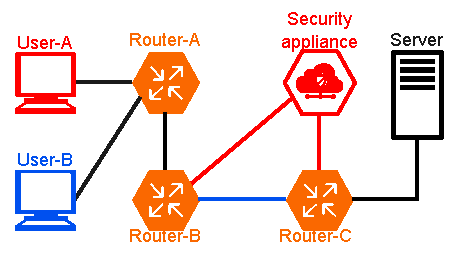
\includegraphics[width=0.95\linewidth]{img/ExplainSrcRtng.pdf}
    \caption{Explain Source Routing}
    \label{fig:exp-src-rtng}
\end{figure}

\subsection*{OpenFlow}
\label{sbsection:openflow}
OpenFlow では,OpenFlow スイッチと呼ばれる OpenFlow に対応した専用の機材をパケットを転送するノードとして使用し,OpenFlow コントローラと呼ばれる専用のマシンが OpenFlow スイッチの経路情報を集中管理する.
OpenFlow のアーキテクチャは一般のパケットルーティングアーキテクチャとは大きく異なる.
一般的なネットワークでは先に挙げた BGP や OSPF などのルーティングプロトコルを利用して経路情報を交換し,ルーティングテーブルを作成する.
そして,ルータは自身が作成したルーティングテーブルに基づいてパケットを転送する.
対照的に,OpenFlow では BGP や OSPF などのルーティングプロトコルを利用してルーティングテーブルを作成することはしない.
経路情報は OpenFlow コントローラが集中管理し,OpenFlow コントローラは自身が決定した経路情報を実際にパケットを転送する OpenFlow スイッチへインストールする.
また,OpenFlow ではルーティングテーブル自体も一般的なルーティングで作成されるものとは異なり,OpenFlow で利用されるルーティングテーブルに対応するテーブルのことをフローテーブルという.
OpenFlow のフローテーブルには,宛先の IP アドレスだけではなく,送信元アドレスや通信を受信したポート,独自定義の専用パケットヘッダのフィールドなどもマッチングルールとして含まれる.
これにより,IP 的なベストパスによらずに,かつ同じ宛先であっても別のパスを選択できる.

\subsection*{NSH}
\label{sbsection:nsh}
NSH は,SFC を実現する 1 つの手法として考えられたプロトコルで,NSH と呼ばれるヘッダでパケットをカプセル化する.
OpenFlow が汎用的なパケット転送アーキテクチャとして考案されたのとは対象的に,NSH は SFC を前提として考案された.
NSH で転送されるパケットの構造を図~\ref*{fig:nsh}として示す.
NSH パケットは,大きく分けて 3 のパートに分けられる.
Original Packet は,実際のエンドツーエンドでやり取りするパケットのことを指す.
そのパケットを,NSH でカプセル化している.
NSH の中にはいくつかのフィールドが存在し,その中には SFC の中でどのパスを通過するのか通過するのかや,ユーザ定義のメタデータ,オプショナルなフィールドなどが含まれる.
NSH でカプセル化されたパケットを,更に Transport Encapsulation というヘッダがカプセル化している.
この Transport Encapsulation は特定のフォーマットである必要はなく,GRE,VXLAN などの一般的なトンネリングプロトコルや通常のイーサフレームである.
Transport Encapsulation の目的は,オーバーレイネットワークを通じて適切な SF ノードまでパケットを転送することである.
NSH に対応したノードでは,SF が適用されたパケットに対して,そのパケットの NSH を参照し次の SF のノードを決定する.
次の SF ノードが決まったらそのノードに届くよう,対応する Transport Encapsulation でカプセル化することで TE ができる.
\begin{figure}[t]
    \centering
    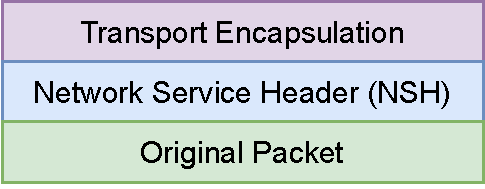
\includegraphics[width=0.95\linewidth]{img/nsh.pdf}
    \caption{Structure of NSH}
    \label{fig:nsh}
\end{figure}

\subsection*{MPLS}
\label{sbsection:mpls}
MPLS とは Multiprotocol Label Switching の略称であり,MPLS ヘッダに含まれるラベル情報に基づいてパケットを転送するプロトコルである.
MPLS ヘッダは Layer 2 ヘッダと Layer 3 ヘッダの間に挿入され,MPLS ヘッダの中にラベル情報を始めとするいくつかのフィールドが埋め込まれる.
MPLS では,宛先の IP アドレスではなく,MPLS ヘッダに含まれるラベル情報を参照してパケットを転送する.
つまり MPLS では,MPLS ヘッダ内に埋め込まれたタグ情報を使ってパケットを転送するため,IP 的なベストパスによらないルールでパケットを転送できる.
また,MPLS は古くから VPN を構成するために用いられてきた一般的なプロトコルである.
そのため,多くのネットワーク機器でサポートされている.
OpenFlow は特別な機器やコントローラが必要であり,NSH も比較的新しいプロトコルで,かつ機能も SFC に特化しているため,NSH をサポートする機材は少ない.
対象的に MPLS は既に多くの機器でサポートされているため,OpenFlow や NSH と比較して導入が容易であるという特徴を持つ.
また,RFC8595~\cite{rfc8595} のように,NSH と MPLS を組み合わせて SFC を実現する手法も提案されている.
このアーキテクチャでは,NSH の Transport Layer として MPLS を利用している.

\section{SRv6}
\label{section:srv6}
先に挙げた技術だけではなく,Segment Routing over IPv6 (SRv6) も TE を適用できる技術の 1 つである.
MPLS が独自のラベルを使って使ってパケットを転送するアーキテクチャであるのに対し,SRv6では MPLS のラベルに対応する概念として IPv6 アドレスを利用する.
SRv6 で利用される識別子はセグメント識別子 (SID) と呼ばれ,各 SID はネットワーク内の特定の場所で実行される特定の機能を表す.
この SID は IPv6 と全く同じフォーマットをしている.
SRv6 では,SRv6ヘッダ (SRH) と呼ばれる IPv6 拡張ヘッダに SID の一連の集合からなるリストを埋め込むことで,ネットワークオペレータやアプリケーションはパケットが通過する中間地点を指定できる.

SRv6 ヘッダには通過するネットワーク上のノードの順番がリストとして埋め込まれ,ルータはそのリストに基づいてパケットを転送する.
図~\ref*{fig:srv6} において,例えば SID リストの要素が \textbf{A,FW,C} である場合,パケットは緑色のパスを通るように転送される.
また,SRv6 はあるパケットが経由するノードを指定できるだけでなく,パケットに対してパケットに対して特定の操作を適用できる.
このようなパケット操作の種類のことを \textbf{SRv6 ビヘイビア} という.
現在 RFC8986~\cite{rfc8986} では 15 種類の End ビヘイビアが定義されている.

\subsection*{SRv6 を利用した layer-3 VPN の構築例と SRv6 によるパケット転送の具体的な動作}
\label{sbsection:srv6-vpn}

SRv6 ビヘイビアを組み合わせることで,layer-3 VPN を構成することもできる~\cite{rfc9252}.
SRv6 を利用した layer-3 VPN の動作を図~\ref*{fig:srv6-vpn} に示す.
図~\ref*{fig:srv6-vpn} \circled{1} において,PE-1 は受信したパケットを SRH でカプセル化する.
このように SRH でパケットをカプセル化する,という操作も SRv6 ではビヘイビアとして定義されており,この操作のことを H.Encaps という.
ここでは,PE-1 は受信したパケットに対して \textbf{A,FW,C} を意味する SID リストを付加したものとする.
このとき,SRv6 でカプセル化されたパケットの宛先アドレスは,内部パケットの宛先アドレスに関わらず,次に到達すべきノードを示す SID である FW Service になる.
PE-1 は H.Encaps で SRH を付加したパケットを Router-A へ送信する.
このとき,パケットは宛先 IPv6 アドレスが Router-A である単なる IPv6 パケットとして扱われる.
PE-1 は自身の持つルーティングテーブルを参照し,Router-A へのネクストホップを決定し,パケットを送出する.
図~\ref*{fig:srv6-vpn} \circled{2} は,Router-A が受信したパケットに対して SID を 1 つ進めて FW Service にパケットを転送している様子を示している.
リスト状になっている SID の中でどれが現在有効な SID であるかを指定するために,SRH にはセグメントレフト (segleft) と呼ばれるフィールドが定義されている.
segleft は SID リストのインデックスであり, $(SID の合計)-1$ から始まり,$0$ で終わる.
Router-A は受信した SRv6 パケットの segleft を 1 つデクリメントし,FW Service の SID が次に有効な SID であることを示すようにする.
また,Router-A はパケットの宛先アドレスを新しく有効になった FW Service の SID に書き換える.
このように,segleft を 1 つ進め,宛先アドレスを新たに有効になった SID で書き換える動作のことを End ビヘイビアといい,これも SRv6 ビヘイビアの 1 つである.
End ビヘイビアは SRv6 の中で最も基本的なビヘイビアである.
宛先アドレスを書き換えたあと,Router-A は自身のルーティングテーブルから新たな宛先アドレス (FW Service の SID) を検索し,ネクストホップへ転送する.
図~\ref*{fig:srv6-vpn} \circled{3} では,\circled{2} と同様に FW Service が End ビヘイビアを実行して segleft デクリメントし,新たに有効になった SID に基づいて Router-C へパケットを転送している.
図~\ref*{fig:srv6-vpn} \circled{4} では,PE-2 が受信したパケットに対して End.DT4 というビヘイビアを実行している.
このビヘイビアは,SRH を取り除き,特定の VRF を参照して SRv6 でカプセル化されていた内部パケットを転送する,という動作を実行する.
End.DT4 により,パケットから SRH は取り除かれ,PE-1 でカプセル化される前のパケットを得ることができる.

\subsection*{SID の構造と構造的な利点}
\label{sbsection:srv6-sid-struct}
先に述べた通り,SID は SRv6 で利用される識別子であり,SRH にはいくつかの SID がリスト状になって含まれる.
図~\ref*{fig:exp-src-rtng} で示されているように,SID は \texttt{LOC:FUNCT:ARG} という 3 つのパートに分かれている.
また,SID は IPv6 アドレスであるため,それら 3 つパートの長さの合計は 128bit である.
\texttt{LOC} はロケータを表す.ロケータとは,ある SID に対応するノードの場所を表す.
\texttt{FUNCT} は SID に関連付けられた SRv6 ビヘイビアの識別であり,\texttt{ARG} はビヘイビアの動作に必要な追加情報をエンコードする領域である.
例えば,End.DT4 では \texttt{ARG} フィールドにはルックアップするべき VRF テーブルを識別するための情報がエンコードされる.

% SRv6 ノードは,宛先 IPv6 アドレスがノードに設定されたローカル SID であるパケットを受信すると,SID に関連付けて事前定義された動作を実行する.
% SRv6 のコンテキストにおいて,SRv6 ノードが実行するパケット操作は End ビヘイビアと称される.
% 現行の RFC8986~\cite{rfc8986} では,15 種類の End ビヘイビアが定義されており,その中で最も基本的なものは End である.
% End ビヘイビアは,受信したパケットの SRH の segleft をデクリメントし,宛先 IPv6 アドレスを次の SID に置換する.
% 続いて,SRv6 ノードは更新された宛先 IPv6 アドレスに基づき,パケットを次のホップに転送する.
% また,RFC8986 では,SID リストを含む SRH でパケットをカプセル化する動作も定義されており,これは Headend ビヘイビアと呼ばれる.
SRv6 の SID は IPv6 アドレスであるため,既存のルーティングプロトコルを用いて SID を経路情報として既存のルーティングプロトコルを利用して広告できる.
SRv6 ビヘイビアは,SID の \texttt{FUNCT} パートで表現される.
しかし,「特定の SRv6 ビヘイビアならば \texttt{FUNCT} パートはこの値である」というようなルールは存在しない.
つまり,SRv6 ビヘイビアの定義は IS-IS の TLV の Type フィールドのようなものとは異なり,ビヘイビアに対応する値は標準化されず,オペレータが自由に決めることができる.
図~\ref*{fig:srv6-vpn} \circled{4} では,Router-C は受信したパケットに対して End.DT4 を実行している.
Router-C は \texttt{LOC:FUNCT:ARG} のフォーマットに従って [Router-C のロケータを示すブロック]:[Router-C 上で End.DT4 として定義されたブロック]:[利用可能な VRF table 番号] を自由に決定し,それを経路情報として周りのノードへ広告する.

SRv6 ビヘイビアが実装されていないネットワーク機器が SRv6 でカプセル化されたパケットを受信した際,その機器は SRv6 パケットを IPv6 パケットとして転送できる.
SRv6 が IPv6 拡張ヘッダを利用したプロトコルであるため,そのパケットは IPv6 パケットとして認識されるからである.
つまり,SRv6 ビヘイビアを実行せず,単にパケットを現在有効な SID へ転送するだけであれば,IPv6 パケットフォワーディングが実装されていれば適切にパケットを転送できる.

% SRv6 ベースのネットワーク構築が可能である.
% 例えば,H.Encaps と End.DT4 はそれぞれヘッドエンドビヘイビア及びエンドビヘイビアに該当し,これら2つのビヘイビアを組み合わせることで layer-3 VPN を構成できる~\cite{rfc9252}.
% H.Encaps は IPv4 または IPv6 パケットを SRH を含んだ IPv6 ヘッダで包み,一方 End.DT4 は SRH でカプセル化されたパケットの外部ヘッダを外す.
% このようにパケットを新たな外部ヘッダで包むことをカプセル化と称し,包まれた外部ヘッダを取り外して内部のパケットを取り出すことをデカプセル化と称す.
% 入口となる SRv6 ノードでは, H.Encaps が出口側 SRv6ノードの End.DT4 SID に対応する IPv6 アドレスを宛先として持つ IPv6 ヘッダで,送信するパケットをカプセル化する.
% 該当パケットは SRv6 ルーティングインフラを通じて,End.DT4 SID の \texttt{LOC} に沿って出口 SRv6 ノードへと転送される.
% SID は IPv6 アドレスであるため,通信の途中の経路ではカプセル化された外側の IPv6 ヘッダの宛先アドレスに基づいてルーティングされる.
% 出口 SRv6 ノードがパケットを受信すると,そのノードは End.DT4 を実行する.
% End.DT4 を実行するとパケットはデカプセル化され,内部パケットは SID の \texttt{ARG} に関連付けられた VRF (Virtual Routing and Forwarding) テーブルに基づいてルーティングされる.

\begin{figure}[t]
    \centering
    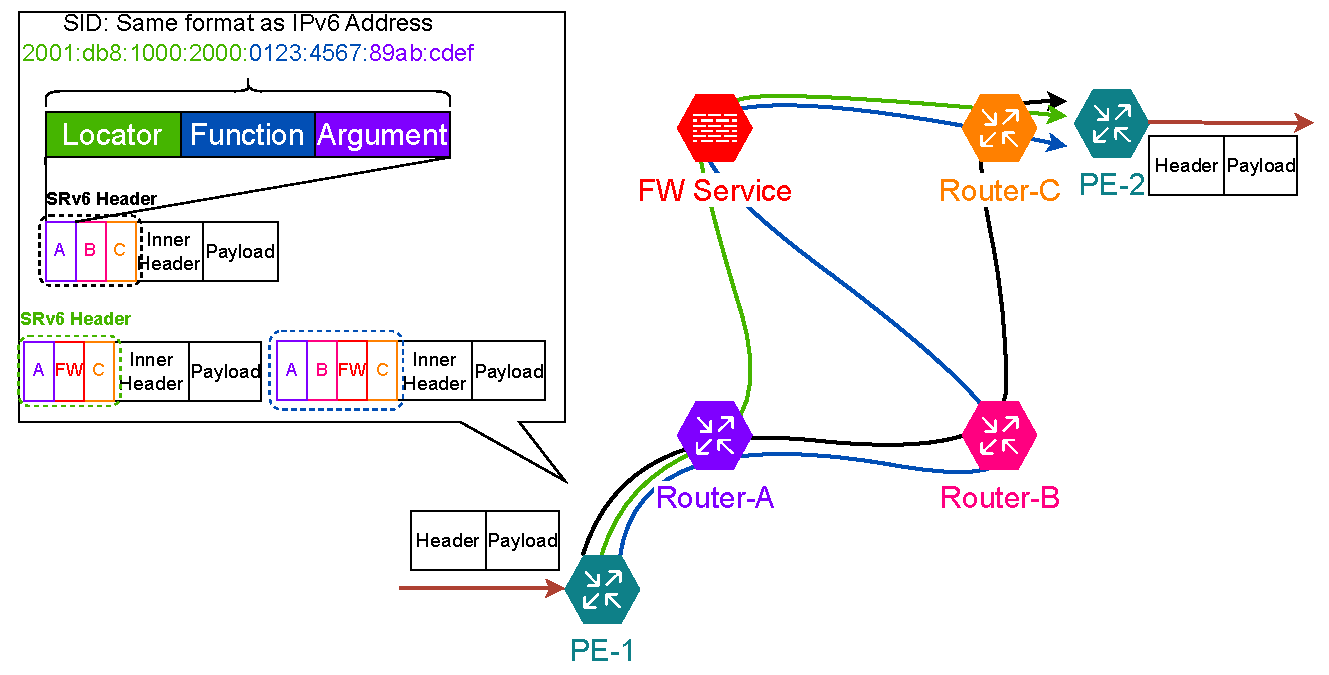
\includegraphics[width=0.95\linewidth]{img/SRv6Arch.pdf}
    \caption{Architecture of SRv6}
    \label{fig:srv6}
\end{figure}

\begin{figure}[t]
    \centering
    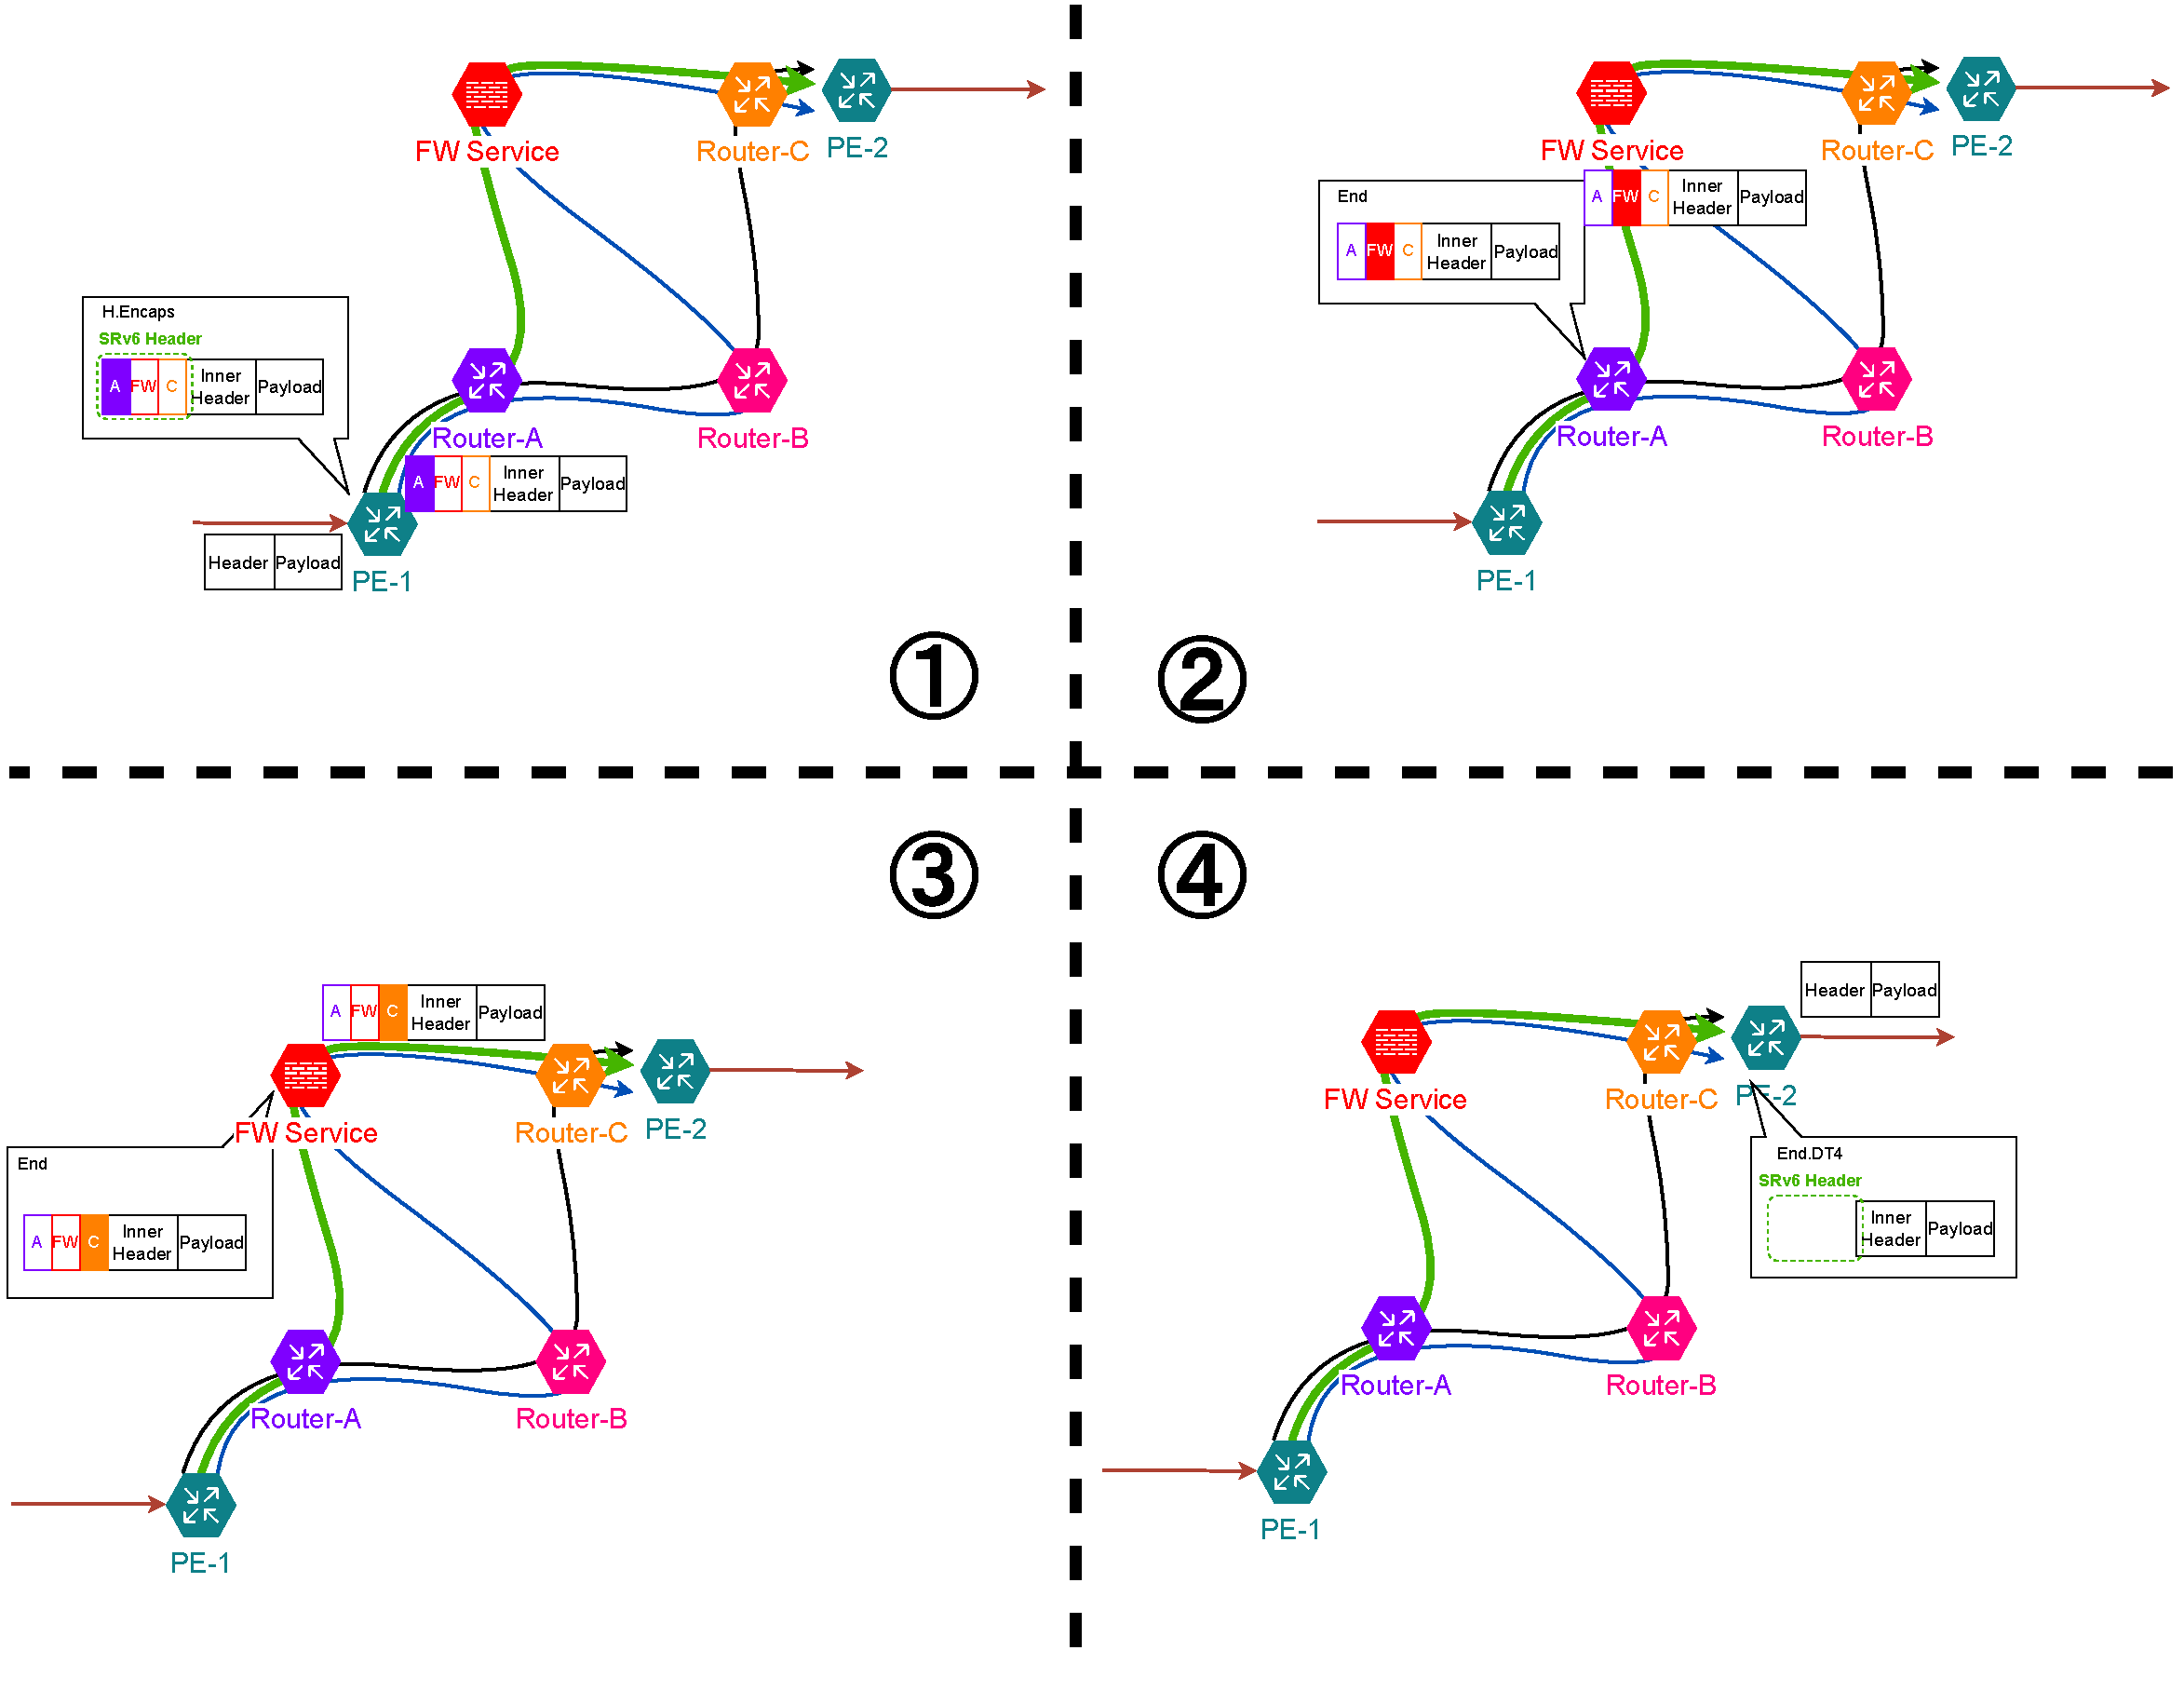
\includegraphics[width=0.95\linewidth]{img/ExplainEndDT4.pdf}
    \caption{layer-3 VPN with SRv6}
    \label{fig:srv6-vpn}
\end{figure}

\section{導入}
\label{section:background}
Service Function Chaining (SFC) は,Software Defined Network (SDN) 及び Network Function Virtualization (NFV) の文脈で研究されているトピックである~\cite{nfv,sfc-on-sdn-nfv-servey,sfc-on-sdn-scenario,imple-sfc-with-openflow}.
SFC では,ネットワーク機能 (NF) を通過する順序や NF のタイプに関する情報を事前に定義し,それらのルールをネットワーク機器に配布する必要がある.
SFC ネットワークを構築するネットワーク機器は,事前に決定されたルールに従って受信したパケットを NF に導く.
パケットを NF へ導くためのルールは,SDN コントローラやルーティングプロトコルによってネットワーク機器に配布される.
ネットワーク機器は IP ルーティング上の最短経路に関係なく,配布された SFC ルールに従ってパケットを転送する次のホップを選択する必要がある.
また,パケットのヘッダにこれらのルールに合致させるための特別な情報を埋め込む手法が取られることもある.
SFC は,クラウドサービスプロバイダ (CSP),アプリケーションサービスプロバイダ (ASP) 及びインターネットサービスプロバイダ (ISP) にとって,現在の静的な環境に代わる柔軟かつ経済的な選択肢を提供する~\cite{survey-on-sfc}.

SFC を実現可能な技術には,いくつかの候補が存在する.
例えば OpenFlow~\cite{openflow},Network Service Header (NSH)~\cite{rfc8300},MPLS~\cite{rfc8595}などである.
これらの技術はどれも,最短経路に関係なく,ルールに基づいて受信したパケットを意図した NF に導く,という要件を満たすことができる.
OpenFlow では,経路情報を管理する中央のコントローラが,実際にパケットを転送する OpenFlow スイッチに対して明示的にパケット転送ルールを設定する.
OpenFlow スイッチは,コントローラによって適切に管理されたルールに従い,パケットを意図した NF に転送する.
OpenFlow のもつこのアーキテクチャは,従来のルーティングプロトコルに基づかない柔軟な経路制御を可能にする.
NSH は Service Path Identifier (SPI) とService Index (SI) によって NF を識別する.
NSH ノードは,パケットに付与された NSH 内の SPI,SI に基づいてパケットを転送する.
NSH は,サービスプレーンと呼ばれる専用のオーバーレイネットワークを作成し,そのオーバレイネットワーク内でサービスを転送する.
このオーバレイネットワークを構築する,というアーキテクチャにより,NSH では基礎となるネットワークトポロジを変更することなくサービス転送を可能にする.
一方,MPLS では,直接 NSH を使用する代わりに,MPLS ラベルスタックを利用する.
このラベルスタックには,パケットが通過すべきノードの順序がホップバイホップで含まれている.
ラベルスタック内で表現されるノードはルータだけでなく,NF も含まれるため,そのラベルスタックに基づいてパケットを転送する事で SFC を実現できる.
このアプローチもまた,基礎となるネットワークトポロジを変更せずに SFC を実現するために必要な,最短経路によらないパケット転送を達成する.

Segment Routing (SR),特に Segment Routing over IPv6 (SRv6) もまた,SFCを実装するために使用される技術の1つである.
SR では,リンク,ノード,サービスといったネットワーク内の各エンティティを\textbf{セグメント}として表現する.
SRv6 パケットのヘッダ (SRH) には,セグメントリストと呼ばれる,そのパケットが通過すべきセグメントの順序を示したリストが含まれている.
SRv6 では,セグメントを識別するための ID (SID) として,IPv6 アドレスを使用する.
言い換えれば,SRv6 は IPv6 ルーティングインフラをその基盤として利用し,SRH 内で定義された順序に従って,任意のセグメントを経由してパケットを転送する.
SRv6 は,NF が実行されるノードをセグメントとして表現し,SID を割り当て,任意の順序で NF を通過するようにパケットを転送することで SFC を実現する.

SRv6 では,NF を SID で表し,セグメントリストに基づいて適切にパケットを転送をすることで,SRv6 を基盤とした SFC ネットワークを実現できる.
しかし,SRv6 レイヤよりも上位にある NF の振る舞いと,基盤となる IPv6 ルーティングインフラをどのように統合するかは明確でない.
例えば,IPv4パケットの Network Address Translation (NAT) を SRv6 ネットワーク内の NF として考慮する場合を考える.
SRv6 ネットワーク内において,IPv4パケットは,SR Header (SRH) を含む外部 IPv6 ヘッダでカプセル化される.
NF で動作する NAT の実装が SRv6 に対応していない場合,SR プロキシ~\cite{ietf-spring-sr-service-programming-08}が必要となり,ネットワーク構成や運用における複雑さが増加してしまう~\cite{draft-scexp}.
実装が内部パケットへの NAT と SRv6 に則した転送動作を同時に実行できる場合,それはレイヤバイオレーションとなる. 
Linux には,SERA~\cite{sera} という iptables を拡張したファイアウォールアプリケーションが存在する.
SERA は SRH でカプセル化されたパケットについて,カプセル化された内部パケットのヘッダ情報にマッチする iptables のフィルタールールを適用できる.
SRv6 での基本的な転送動作として,End と呼ばれる動作がある.
SERA は iptables を拡張することで,この End 動作を処理する機能も実装されている.
ただし,既にLinux カーネルには IPv6 ルーティング,及び SRv6 End 動作に関する処理が実装されている.
SERA は,Linux カーネルに実装されている SRv6 機能を使わずに,独自に改良した iptables アクションによって End 動作を処理する.
つまり,SERA は Linux カーネル内で統合されている IPv6 ルーティングインフラと SRv6 処理機能を使わずに,独自に拡張した iptables によって SRv6 とフィルタリングサービスとしての NF を統合している.

本論文では,既存の netfilter ベースアプリケーションの実装を変更することなく SRv6 対応 NF として扱えるようにする,End.AN.NF 提案する.
End.AN.NF は Linux netfilter を NF として扱えるようにしつつ,Linux に実装されている IPv6 ルーティングインフラを活用する.
End.AN.NF は受信した SRv6 内部パケットに対して,netfilter のフックポイントを透過的するように設計されている.
本論文では End.AN.NF を Linux カーネル上で実装し,スループットとレイテンシを評価した.
評価の結果,End.AN.NF は End.DT 4と H.Encaps の組み合わせによる SRv6 内部パケットへの netfilter 適用と比較し て27\% 高いスループットと 3.0 マイクロ秒低いレイテンシを実現した.
さらに,End.AN.NFのレイテンシは,End.DT4とH.Encapsの組み合わせよりも3.0マイクロ秒低い.
また,End.AN.NFのレイテンシはマイクロ秒解像度でEnd動作と同じである.

\section{本論文の目的と構成}
本論文における以降の構成は次の通りである.
\ref*{chap:introduction}章では,本論文の構成,及び本論文の概要を述べる.
\ref*{chap:related_works}章では,サービスファンクションチェイニングに関する前提知識,及びそれを実現する技術について解説し,本論文の概要について述べる.
\ref*{chap:design_and_impl}章では,本論文の提案する新たな SRv6 End behavior である End.AN.NF についての詳細な動作,及び実装について述べる.
\ref*{chap:evaluation}章では,実装した End.AN.NF について,レイテンシ及びスループットの性能を特定のを変化させながら性能の計測する.
\ref*{chap:conclusion}章では,本研究における結論と今後の展望について述べ,End.AN.NF に必要なネットワーク制御プレーンについて検討する.